\section{Implementation and evaluation}\label{sec:experiment}
In this section, an experimental evaluation over three real-life event logs is reported.
The aim of the evaluation is to measure to what extent the forecasted process models/DFGs are capable of correctly reproducing actual future DFGs in terms of allowing for the same process model behaviour.
To this purpose we benchmark the actual against the forecasted entropic relevance discussed in \Cref{sec:2:motivation}.
This is done at various parts of the trace, i.e. forecasts for the middle of the event logs up to the later parts of the event log to capture the robustness of the forecasting techniques in terms of the amount of data required to obtain good prediction results for both the equisized and equitemporal aggregation.

\subsection{Re-sampling and test setup}
To obtain training data, time series are obtained by specifying a number of intervals (i.e. time steps in the DF time series) using either equitemporal or equisized aggregation a described in Section \ref{sec:3a:preliminaries}.
Time series algorithms are parametric and sensitive to sample size requirements \cite{hanke2001business}.
Depending on the number of parameters a model uses, a minimum size of at least 50 steps is not uncommon, although typically model performance should be monitored at a varying number of steps.
In the experimental evaluation, the event logs are divided into 100 time intervals with a varying share of training and test intervals. A constant and long horizon $h=25$ is used meaning all test sets contain 25 intervals, but the training sets are varied from $ts=25$ to $ts=75$ intervals, meaning the forecasts progressively target the prediction of intervals 25-50 (the second quarter of intervals) over to 75-100 (the last quarter of intervals).
This allows to both inspect the difference in results when only few data points are used, and whether there is a difference forecasting data points in the middle or towards the end of the available event data.

Resampling is applied based on a 10-fold cross-validation constructed following a rolling window approach for all horizon values $h\in[1,25]$ where a recursive strategy is used to iteratively obtain $\hat{y}_{t+h|T_{t+h-1}}$ with $(y_1,\dots,y_{T},\dots,\hat{y}_{t+h-1})$ \cite{weigend2018time}.
10 training sets are hence constructed for each training set length $ts$ and exist from $(y_1,\dots,y_{T-h-f})$ and the test sets from $(y_{T-h-f+1},\dots,y_{T-f})$ with $f\in[0,9]$ the fold index \cite{bergmeir2012use}.
While direct strategies with a separate model for every value of $h$ can be used as well and avoid the accumulation of error, they do not take into account statistical dependencies for subsequent predictions.

Three popular publicly-available event logs are used: the 2012 BPI challenge log\footnote{\url{https://doi.org/10.4121/uuid:3926db30-f712-4394-aebc-75976070e91f}}, the Sepsis cases event log\footnote{\url{https://doi.org/10.4121/uuid:915d2bfb-7e84-49ad-a286-dc35f063a460}}, and the Road Traffic Fine Management Process log (RTFMP) event log (see Section \ref{sec:2:motivation}.
Each of these logs has a diverse set of characteristics in terms of case and activity volume, as well as average trace length, as can be seen in Table \ref{tab:eventlogs}.
\begin{table}[htbp]
  \centering
    \begin{tabular}{lrrr}
    \toprule
    \textbf{Event log} & \multicolumn{1}{l}{\textbf{\# cases}} & \multicolumn{1}{l}{\textbf{\# activities}} & \multicolumn{1}{l}{\textbf{Average trace length}} \\
    \midrule
    \textbf{BPI 12} & 13,087 & 36    & 20.020 \\
    \textbf{Sepsis} & 1,050 & 16    & 14.490 \\
    \textbf{RTFMP} & 150,370 & 11    & 3.734 \\
    \bottomrule
    \end{tabular}%
  \caption{Overview of the characteristics of the event logs used in the experimental evaluation.}
  \label{tab:eventlogs}%
\end{table}%

%An example of applying the equisized or equitemporal aggregation to the Sepsis event log with 100 intervals results in the DF time series of Figure \ref{fig:sepsists}, where the DF occurrences of the most frequently occurring activity pair is included.
%For the equisized aggregation, the number of DFs is indeed relatively stable over the log's timeline where for the equitemporal aggregation a noticeable decline of DF pairs is visible towards the end of the series.
%This phenomenon is typical in event logs, as processes usually have particular endpoint activities, but can also be due to the unequal distribution of events over the event log's time line.
There are a few considerations concerning the DF time series in these event logs.
Firstly, DFs of activity pairs containing end point activities (i.e. at the start/end of a trace) often only contain meaningful numbers at very particular parts of the series and are hard to process by longitudinal algorithms which require a longer pattern to extract a meaningful pattern for prediction.
Secondly, especially the equitemporal aggregation can suffer from event logs in which events do not occur as frequently throughout the full log's development.
E.g., the Sepsis log's number of event occurrences tails off towards the end which can be alleviated by pre-processing (not done here to remain consistent over the event logs).
Finally, if the level of occurrences of the DF pair is low and close to 0, the series might be too unsuitable for analysis with white noise series analysis techniques that assume stationarity.
Ideally, every time series is tested using a stationarity test such as the Dickey-Fuller unit root test \cite{leybourne1995testing} and an appropriate lag order is established for differencing. 
Furthermore for each algorithm, especially ARIMA-based models, (partial) auto-correlation could establish the ideal $p$ and $q$ parameters.
However, for the sake of simplicity and to avoid solutions where each activity pair has to have different parameters, various values are used for $p$, $d$, and $q$ and applied to all DF pairs where only the best-performing are reported below for comparison with the other time series techniques.
The results contain the best-performing representative of each forecasting family.
% \begin{figure}[tb]
% 	\centering
% 	\subfigure[Most common DF - equisize]{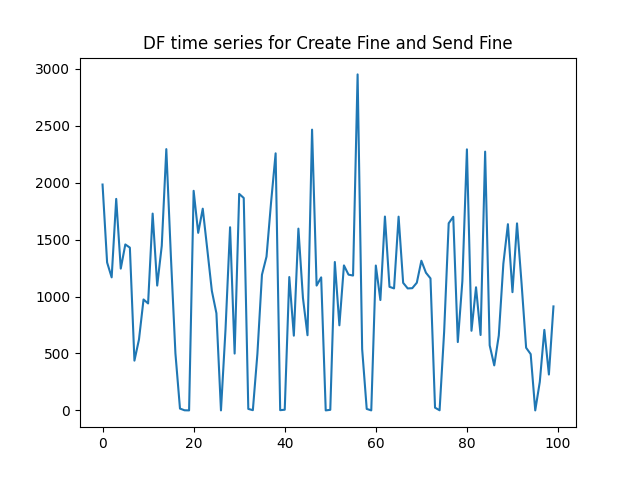
\includegraphics[width=0.39\textwidth]{./img/rtfmp_1.png}}
% 	\subfigure[Most common DF - equitemp]{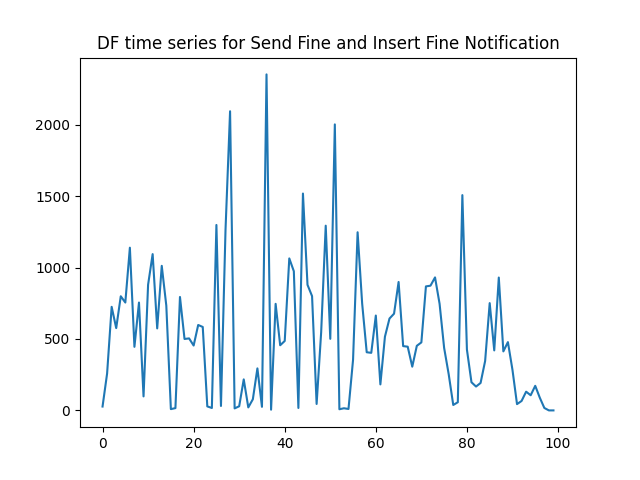
\includegraphics[width=0.39\textwidth]{./img/rtfmp_1_t.png}}
% 	\caption{RTFMP}
% 	\label{fig:sepsists}
% \end{figure}

% \subsection{Evaluation criteria}
% Given that we want to evaluate the capability of the approach to accurately predict the evolution of the process model, the combination of all DF predictions is considered to obtain a global DFG prediction.
% The following two criteria are used:
% \begin{itemize}
% 	\item \textbf{Cosine distance:} measures the distance between two vectors and is often used to compare graph distance. This metric is used to compare the DFGs' edge weight matrices between the actual and predicted number of DF relations.
% 	\item \textbf{Entropic relevance:} see section \ref{sec:2:motivation}.
% \end{itemize}
% These criteria balance a predictive and structural evaluation of the algorithms and report on both the numeric performance common in a forecasting setting as well as their appropriateness in terms of reproducing a structurally usable process model which allows for the observed process behaviour.
% In both cases a lower score is better.

\subsection{Results}
All pre-processing was done in Python with a combination of \emph{pm4py}\footnote{\url{https://pm4py.fit.fraunhofer.de}} and the \emph{statsmodels} package \cite{seabold2010statsmodels}. 
The code and full results are available here\footnote{\url{https://github.com/JohannesDeSmedt/pmf}}.
Figures \ref{fig:equisize} and \ref{fig:equitemp} contain visualisations of the entropic relevance over the predicted intervals for 25, 50, and 75 intervals in the training set respecitively (amounting to 50, 75, 100 intervals used overall with a 25 interval test set). 
It is clear that the actual DFG is lower for all datasets and both aggregation types.
Next, it can be seen that mostly when fewer training points are used there is a more noticeable difference between forecasting techniques.
For longer training sets the differences even out and forecasting techniques perform roughly similar for all datasets and aggregation types with the exception of ARIMA.
Despite the long horizon, the entropic relevance of the predicted models remains relatively stable even further along in the test set.
Only for the equitemporal aggregation on the Sepsis log there is a strong decline towards the end of the event long due to the strong decrease of the number of event occurrences.
\begin{table}[htbp]
  \centering
  \resizebox{0.65\textwidth}{!}{
    \begin{tabular}{|c|l|ccc|ccc|ccc|}
\cmidrule{3-11}    \multicolumn{1}{r}{} &       & \multicolumn{3}{c|}{\textbf{BPI 12}} & \multicolumn{3}{c|}{\textbf{Sepsis}} & \multicolumn{3}{c|}{\textbf{RTFMP}} \\
    \multicolumn{1}{r}{} &       & \textbf{50} & \textbf{75} & \textbf{100} & \textbf{50} & \textbf{75} & \textbf{100} & \textbf{50} & \textbf{75} & \textbf{100} \\
    \midrule
    \multirow{5}[2]{*}{\begin{sideways}\textbf{equisize}\end{sideways}} & \textbf{nav} & \textbf{2.63} & 2.55  & 2.23  & 8.66  & 7.19  & 5.85  & \textbf{35.10} & \textbf{19.63} & 17.03 \\
          & \textbf{arima212} & 4.49  & \textbf{2.31} & \textbf{2.20} & NA    & 8.93  & 6.55  & 40.65 & NA    & 20.71 \\
          & \textbf{ar2} & 2.91  & 2.69  & 2.22  & 10.45 & 6.49  & 5.14  & NA    & NA    & \textbf{14.44} \\
          & \textbf{hw} & 2.71  & 2.41  & 2.22  & 8.25  & 7.52  & 6.20  & 43.06 & 24.09 & 20.20 \\
          & \textbf{garch} & 3.02  & 3.02  & 2.26  & \textbf{7.66} & \textbf{6.14} & \textbf{4.95} & 37.65 & 22.93 & 15.12 \\
    \midrule
    \multicolumn{1}{|c|}{\multirow{5}[2]{*}{\begin{sideways}\textbf{equitemp}\end{sideways}}} & \textbf{nav} & 3.75  & \textbf{3.09} & 3.11  & 9.77  & 6.99  & NA    & 20.81 & 12.96 & 15.19 \\
          & \textbf{arima212} & 5.35  & 4.16  & \textbf{2.83} & 14.87 & 7.88  & NA    & 33.03 & 13.79 & \textbf{14.48} \\
          & \textbf{ar2} & NA    & 3.19  & 3.13  & 15.35 & 6.51  & NA    & NA    & 13.06 & 15.38 \\
          & \textbf{hw} & 4.10  & 3.21  & 3.06  & \textbf{7.98} & 6.08  & NA    & 26.15 & 13.29 & 15.77 \\
          & \textbf{garch} & \textbf{3.74} & 3.19  & 3.17  & 23.00 & \textbf{5.68} & NA    & \textbf{19.68} & \textbf{11.68} & 14.64 \\
    \bottomrule
    \end{tabular}%
    }
    \caption{Overview of the mean percentage error in terms of entropic relevance.}
  \label{tab:result_table}%
\end{table}%


Table \ref{tab:result_table} contains the mean absolute percentage error (MAPE) of the actual and forecasted DFGs to quantify the difference in terms of entropic relevance.
For the BPI12 log, the best-performing predictions are within a 8.5-13\% difference bracket, while for the Sepsis case the differences increase drastically to 80-100\%, and 28-110\% for the RTFMP log when the instable and very high differences on only using 25 intervals in the training set are discarded.
Most algorithms do perform similarly, indicating that even an average naive forecast suffices to outperform more intricate models such as GARCH except for ARIMA and AR models which boast the best results in most cases offering a significantly better performance overall.
One of the reasons for such a difference in error which seems most apparent is the number of activities, given that the BPI12 log has more than twice the amount of activities compared to the other logs. 

\begin{figure}
    \centering
    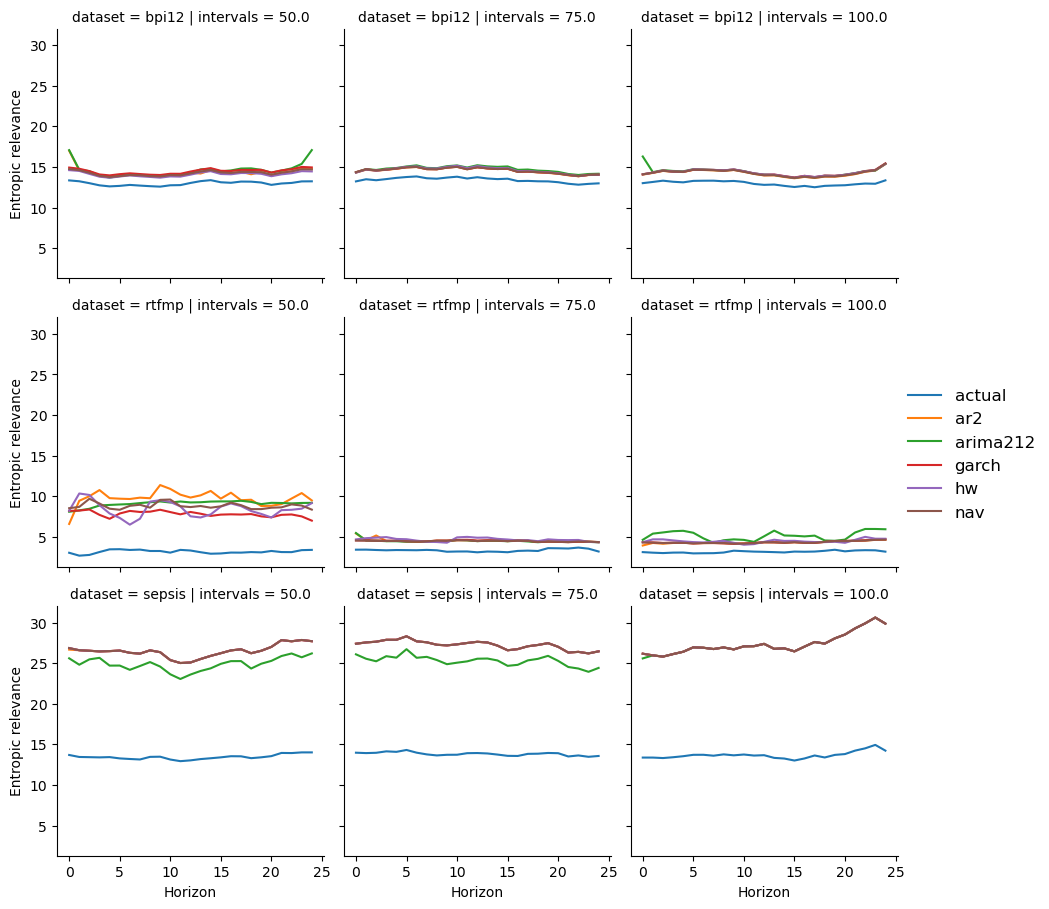
\includegraphics[width=0.8\textwidth]{img/cv_entropic_small_equisize.png}
    % 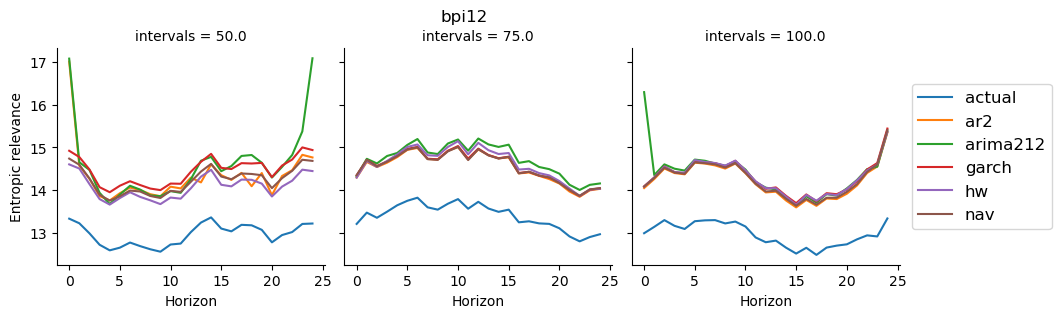
\includegraphics[width=0.8\textwidth]{img/cv_bpi12_entropic_small_equisize.png}
    % 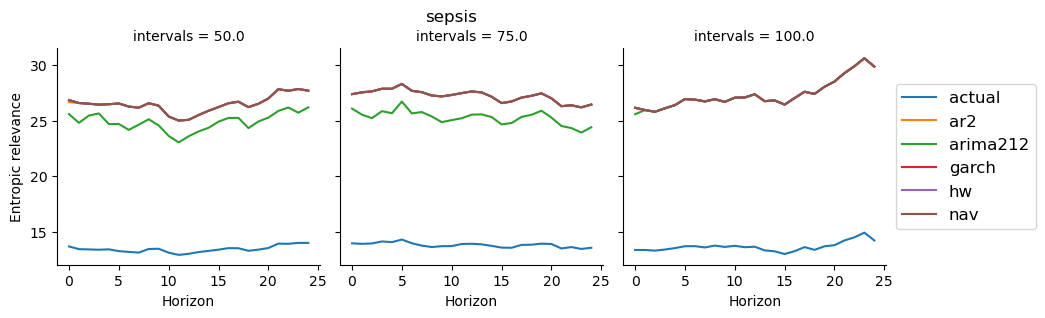
\includegraphics[width=0.8\textwidth]{img/cv_sepsis_entropic_small_equisize.png}
    % 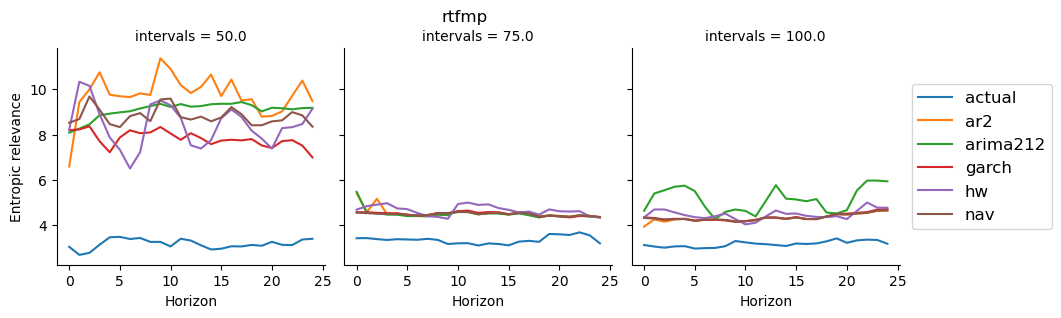
\includegraphics[width=0.8\textwidth]{img/cv_rtfmp_entropic_small_equisize.png}
    \caption{Entropic relevance results for equisize aggregation. Best (lowest) results are indicated in bold.}
    \label{fig:equisize}
\end{figure}
\begin{figure}
    \centering
    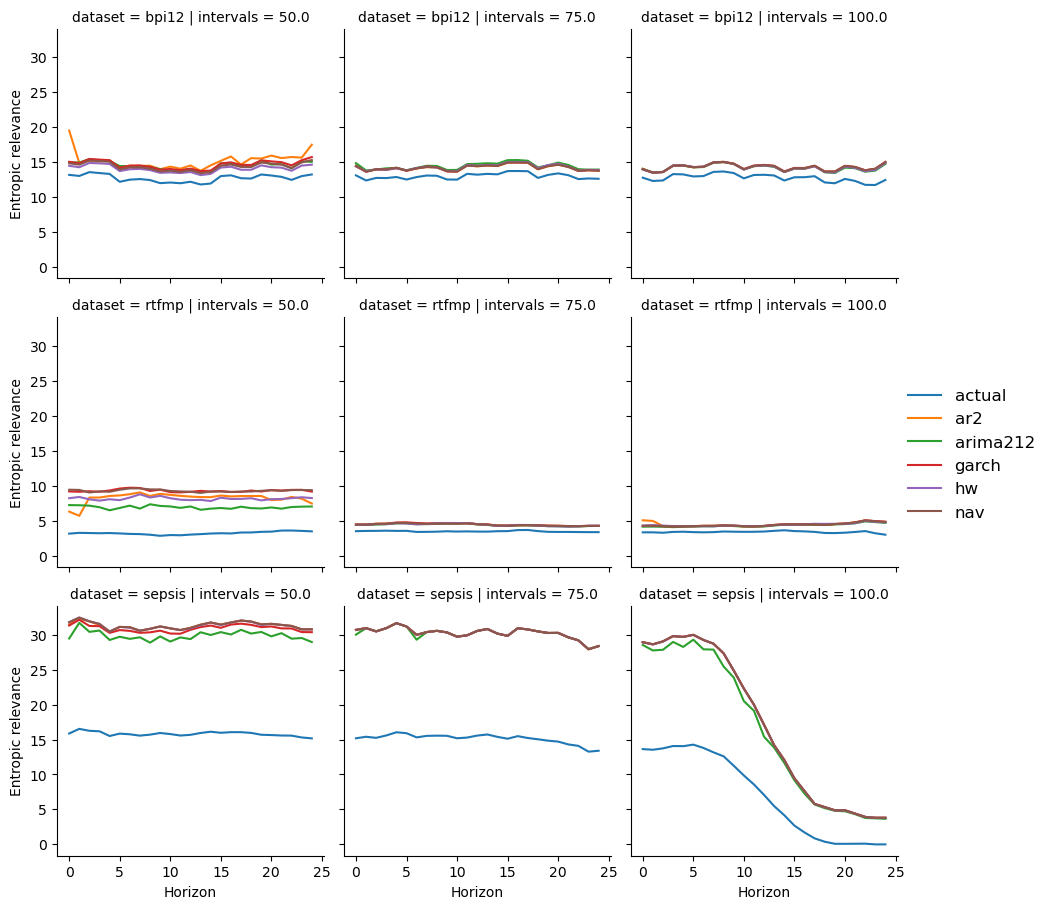
\includegraphics[width=0.8\textwidth]{img/cv_entropic_small_equitemp.png}
    % 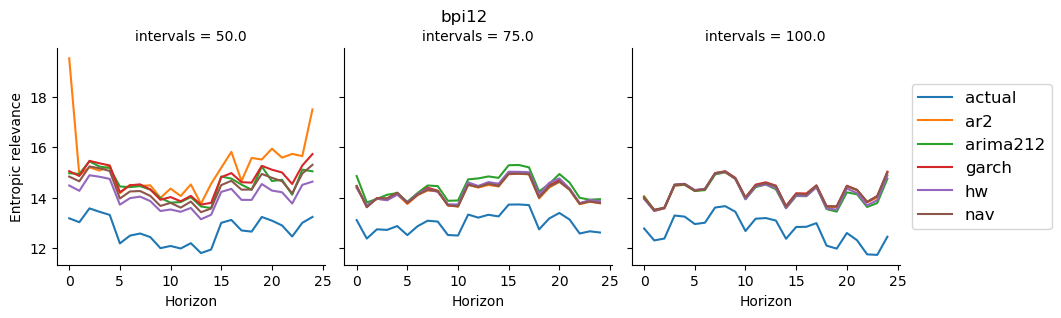
\includegraphics[width=0.8\textwidth]{img/cv_bpi12_entropic_small_equitemp.png}
    % 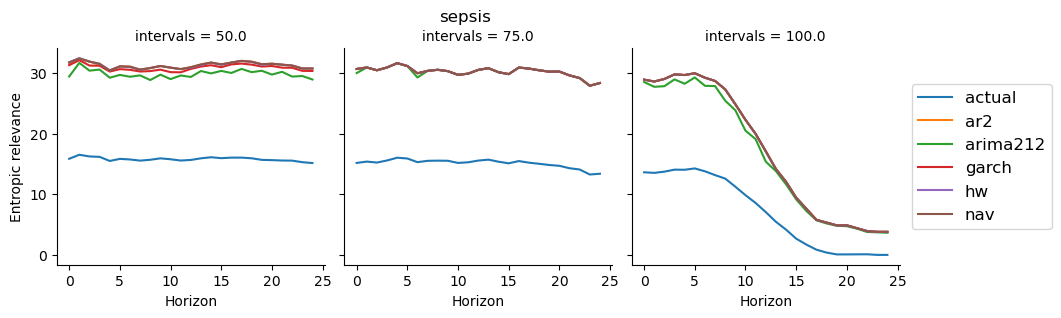
\includegraphics[width=0.8\textwidth]{img/cv_sepsis_entropic_small_equitemp.png}
    % 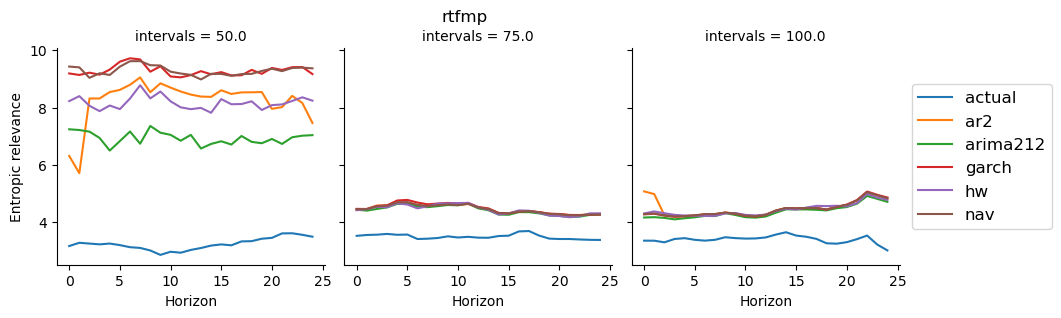
\includegraphics[width=0.8\textwidth]{img/cv_rtfmp_entropic_small_equitemp.png}
    \caption{Entropic relevance results for equitemporal aggregation. Best (lowest) results are indicated in bold.}
    \label{fig:equitemp}
\end{figure}

\subsection{Managerial implications}
Depending on the event log, it is feasible to obtain good (\textless15\%) to very good (\textless5\%) forecasting results in terms of the MAPE and entropic relevance against actual DFGs.
The experiments show that the number of intervals used for training vastly impacts results, which is expected given that with 10-fold cross-validation, this results in only 15 interval being used for the tenth fold to predict the next 25 intervals.
Given that GARCH models often perform strongly suggests that DF time series benefit from the use of models which allow for a varying level of variance.
This makes sense in an event log context, as activities generating the DF occurrences do not occur uniformly during the execution of a process.

\subsection{Visualising Process Model Forecasts}\label{sec:visualisation}

In~\Cref{sec:4.3:results} we evaluated forecasting results, ensuring the conformance and interpretability of the predicted process models. To that end, gaining actual insights from such predicted data remains a difficult task for the analyst. This section sets off to present the implementation of a novel visualisation system to aid analysts in exploration of the event logs. The process of designing and implementing the system started by designing several prototypes that undergone rounds of discussions to mature into the implemented visualisation system. 

The design of the PCE system is shown in Figure~\ref{fig:vis-two-brushes}. It shows an interactive visualisation system with several connected views. The system is implemented with D3.js JavaScript library and is available as an open source project\footnote{See \url{google.com}}.
\todo[inline]{Please check. I went to \url{google.com} and only found a search engine, but a PCE system.}

\begin{figure}
	\centering
	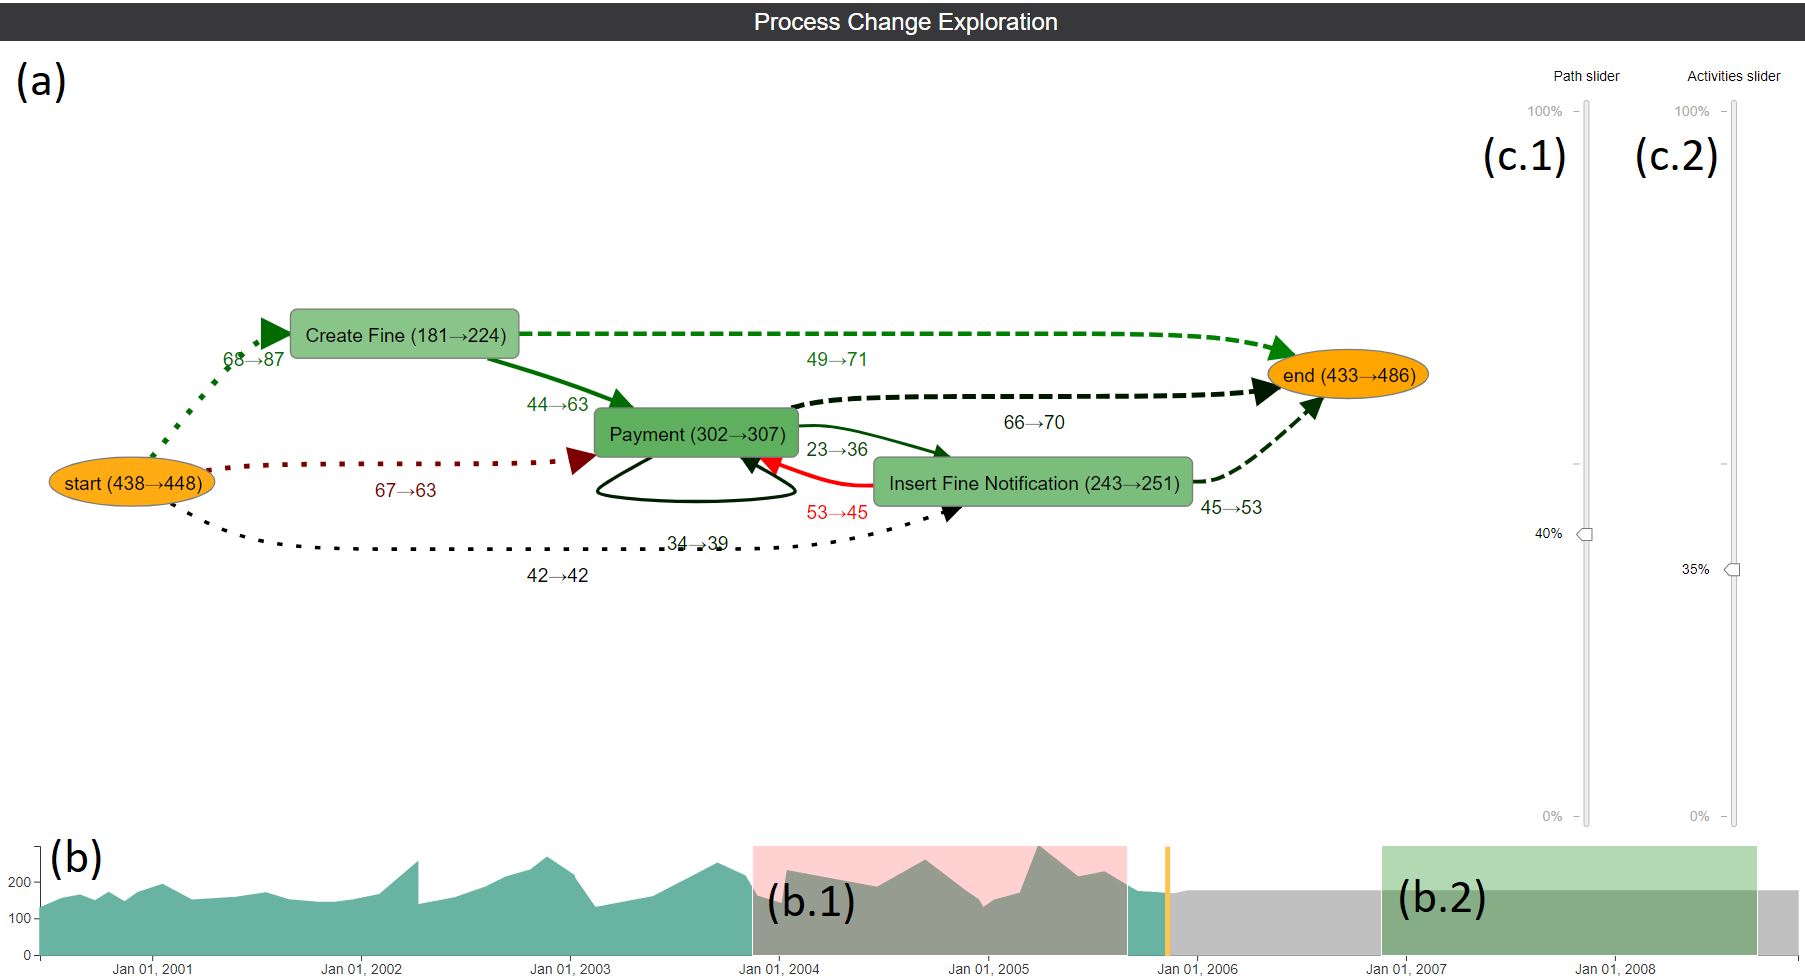
\includegraphics[width=\textwidth]{img/vis/actual-predicted-two-brushed-regions-system.PNG}
	\caption{Process Change Exploration (PCE) system.~\emph{(a)} shows~\emph{Adaptation Directly-Follows Graph (aDFG)} view.~\emph{(b)} shows the \emph{Timeline view with brushed regions} view. Users can brush one or more regions on this graph in order to filter the scope of the analysis~\emph{(b.1}, and~\emph{b.2)}. Two additional views on~\emph{(c)} show the \emph{activity and path sliders}.} 
	\label{fig:vis-two-brushes}
\end{figure}